\begin{refsection}
%-------------------------------------------------------------------------
%-------------------------------------------------------------------------
\chapter{Optical imperfections in refractive lenses}\label{sec:optical_imperfections}
%-------------------------------------------------------------------------
%-------------------------------------------------------------------------

To understand impact of CRL on the optical design of complete beamlines, it is necessary to be able to simulate them realistically. The basic implementation of X-ray lenses is already available on the two most widespread beamline simulation tools: \textit{SHADOW} [\cite{SanchezdelRio2011}] and \textit{SRW} [\cite{Chubar1998}]. Both implementations, although based on different schemes, ray tracing [\cite{Alianelli2007}] and wave optics [\cite{Baltser2011}] respectively, are based on an ideal model combining refraction and absorption for the stacked lenses. Much has been done in terms of refining the modelling of ideal X-ray lenses [\cite{Umbach2008, SanchezdelRio2012, Osterhoff2013, Simons2017, Pedersen2018}] and, to a certain extent, the modelling of optical imperfections [\cite{Pantell2001, Andrejczuk2010, Gasilov2017, Osterhoff2017}]. With exception of the work presented in [\cite{Roth2014}], investigating and simulating the inner structure of X-ray lenses, the present models consider mainly the lens shape and departure from a perfect parabolic shape. The majority of these models, however, is not publicly available, nor are readily compatible with standard beamline simulations suits like \textit{SHADOW} and \textit{SRW}. Another bottle-neck to the current literature or computer codes for simulating CRLs is that they do not include the data from real lenses metrology, as is routinely done for X-ray mirrors simulations [\cite{SanchezDelRio2016}], which undermines the inclusion of CRLs in simulations of complete beamline configurations in combination with other optical elements.

This chapter presents a proposed framework for simulating CRL taking into account not only their thickness and absorption, but also individual lens phase errors. Such phase errors arise from material inhomogeneities (voids, impurities) and/or figure errors from the lens forming process, which can be either modelled based on typical fabrication processes or measured with at-wavelength metrology. The experimental technique used to obtain the lens shape profile in the projection approximation, namely, X-ray speckle tracking, is discussed at length. After considerations on data processing and analysis, a selection of experimental data is discussed and and corrective optics based on the metrology data is proposed. 

%-------------------------------------------------------------------------
%-------------------------------------------------------------------------
\section{Describing and modelling optical imperfections in refractive lenses}
%-------------------------------------------------------------------------
%-------------------------------------------------------------------------

In the paraxial approximation, the parabolic shape for a refracting surface is generally regarded as the ideal shape\footnote{The shape of a focusing refracting surface can be derived from the Fermat's principle, but the parabolic shape is generally regarded as a good approximation. Large apertures are often necessary when very small focused beams are required, but increasing the geometric aperture of the optical element causes the parabolic approximation to under-perform. Several aspheric surface shapes for different focusing conditions were reported in [\cite{SanchezdelRio2012}] - cf. Fig~4. For a deeper discussion on aspheric surfaces in the context of optics, please, refer to [\cite{Schulz1988}].} for minimising aberrations. It is legit, then, to define as errors any deviation from this ideal parabolic shape\footnote{Such definition, however, leaves out discrepancies in the radius of curvature $R$ (designed vs. \textit{de facto}) and the associated defocus it may cause. Discrepancies between designed and executed lenses may render them to be labelled as out-of-specification and may cause the system to under-perform, but are not deviations of the parabolic shape, provided the ideal parabolic shape takes into account the \textit{de facto} radius of curvature. Accounting for such discrepancies can be done using the ideal model described by the transmission element $\mathrm{T}_{\text{single lens}}(\Delta_z)$ (cf. Eq.~\ref{eq:TE_singlelens}) using the \textit{de facto} radius of curvature.} regardless of its origin. The phase errors induced by an ideal lens misalignment will be presented first, then the typical fabrication errors of bi-concave lenses will be presented shortly after. The misaligment and fabrications errors presented in this section were derived from the accumulated experience in handling beryllium and aluminium bi-concave embossed lenses, which are the most available throughout beamlines in diverse synchrotron facilities, however, the modelling presented here is generic enough to be applicable to a wide-range of CRL from diverse fabrication processes\footnote{cf. Table~1 from the supplementary material from [\cite{Roth2017}].}.  
%-------------------------------------------------------------------------
%-------------------------------------------------------------------------
\subsection{Misalignments}
%-------------------------------------------------------------------------
%-------------------------------------------------------------------------

Misalignments of optical systems are not optical errors \textit{per se} if they can be mitigated by ensuring proper alignment is done; they will, however, cause changes to the ideal parabolic phase profile if left uncorrected and will affect the optical performance of the system. Although aligning a CRL stack is possible\footnote{The possibility of realignment of the CRL depends on where and how they are installed in the beamline. If their installation is on a bulky transfocator [\cite{Vaughan2011}], their realignment is more difficult to be performed. However, when used as a final focusing element, enclosed in small casings or compact transfocators - cf. Fig.~3 in [\cite{Lengeler1999}] and [\cite{Kornemann2017, Narikovich2019}], their realignment can be done more easily.}, the individual lenslets usually cannot be aligned in respect to each other, hence the interest in modelling such misalignments.

\begin{figure}[t]
    \centering
    {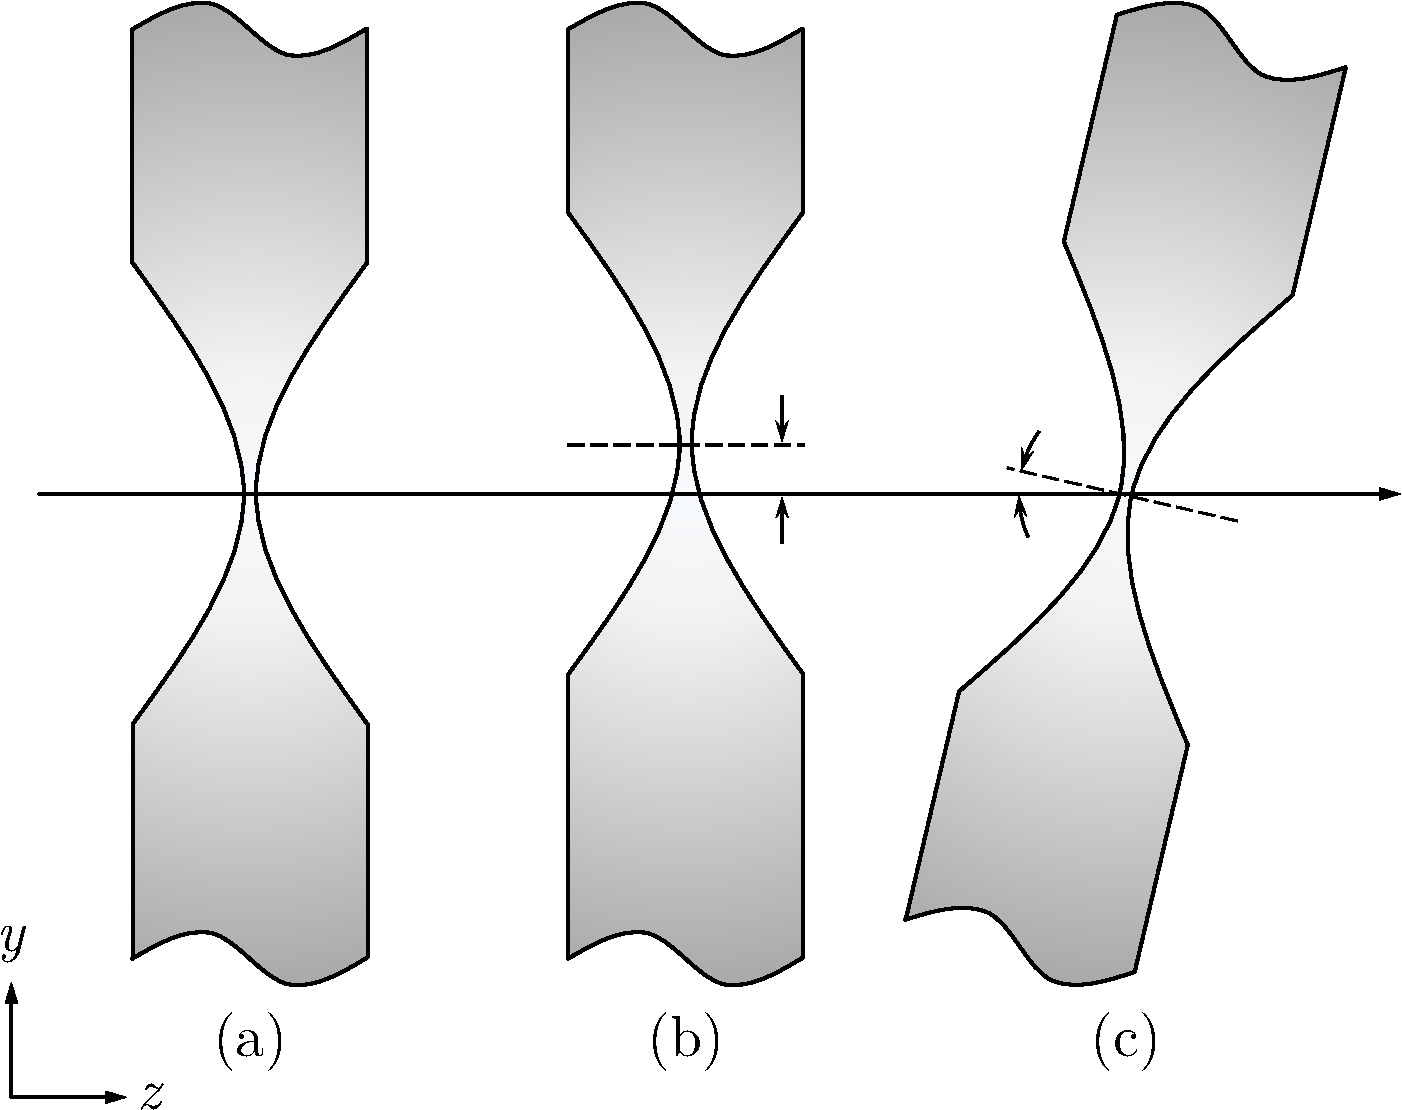
\includegraphics[width=0.4\linewidth]{figures/ch04/missalignments.pdf}}
    \caption[Single lens typical misalignment]{(a) ideal lens for reference. The reference lens not only has a perfect parabolic shape, but is also aligned with the optical axis and centered on the parabolic wavfront; (b) lenslet transverse offset in relation to the optical axis $z$; (c) tilted lens with pivot point between axis of the two parabolic refracting surfaces.}
    \label{fig:missaligments}
\end{figure}

%-------------------------------------------------------------------------
%-------------------------------------------------------------------------
\subsubsection*{Transverse misalignment (lateral offset)}
%-------------------------------------------------------------------------
%-------------------------------------------------------------------------

Shifting transversely a single element an incremental transverse distance $(\Delta_x,\Delta_y)$ can be simply done by calculating $\Delta_z(x-\Delta_x,y-\Delta_y)$ in Eq.~\ref{eq:ProjecThick}. The tilted element is depicted in Fig.~\ref{fig:missaligments}(b). For a pair of coordinates $(x,y)$:
\begin{equation}\label{eq:ProjecThick_misaligned}
    \Delta_z(x-\Delta_x,y-\Delta_y) = 
        \begin{cases}
      \cfrac{(x-\Delta_x)^2}{R_x}+\cfrac{(y-\Delta_y)^2}{R_y}+\text{t}_\text{wall}, &\quad\forall~(x-\Delta_x,y-\Delta_y) \in A,\\
      L, &\quad\text{otherwise}.
        \end{cases}
\end{equation}   
Eq.~\ref{eq:ProjecThick_misaligned} is the ideal parabolic profile of a bi-concave lens given by Eq.~\ref{eq:ProjecThick} with its vertices\footnote{As in optical cardinal points.} centred around $(\Delta_x,\Delta_y)$. While a single transversely shifted lens considered on its own is innocuous, piling up several shifted lenses has considerable impacts on the overall accumulated phase parabolic shape and resulting geometric aperture.

\todo{Work example: a single Be 50um lens shifted. Two Be lenses symmetrically, three Be: a, +Deltax1, -Deltax2 - Example of the axicon.}

%-------------------------------------------------------------------------
%-------------------------------------------------------------------------
\subsubsection*{Angular misalignment (tilted element)}
%-------------------------------------------------------------------------
%-------------------------------------------------------------------------

The angular misalignment of a single lens in space can be described by rotation matrices in three dimensions. The transformation matrices allowing a rotation $\theta$ around each of the Cartesian axis are [\cite[\textit{§C}]{House2016}]:
\begin{subequations}\label{eq:affine}
    \begin{align}
        R_x &= \begin{bmatrix}
                            1 & 0 & 0 &0\\
                            0 & \cos\theta_x & -\sin{\theta_x}  &0\\
                            0 & \sin\theta_x & \cos\theta_x &0\\
                            0 & 0 & 0 &1
            \end{bmatrix}  &&(\small{\text{rotation around the $x-$axis}}),\\
            R_y &= \begin{bmatrix}
                            \cos\theta_y & 0 & \sin\theta_y &0\\
                            0 & 1 & 0 &0\\
                            -\sin\theta_y & 0 & \cos\theta_y &0\\
                            0 & 0 & 0 &1
            \end{bmatrix}  &&(\small{\text{rotation around the $y-$axis}}),\\
            R_z &= \begin{bmatrix}
                            \cos\theta_z & -\sin\theta_z & 0 &0\\
                            \sin\theta_z & \cos\theta_z & 0 &0\\
                            0 & 0 & 1 &0\\
                            0 & 0 & 0 &1
            \end{bmatrix}  &&(\small{\text{rotation around the $z-$axis}}).
    \end{align}
\end{subequations}{}
Matrix multiplication is associative, which implies that if multiple rotations are involved, that is $R_x, R_y$ and $R_z$ are applied to a set of points $(x,y,z)$, an equivalent rotation matrix $R_{\theta}=R_zR_yR_x$ can be calculated and then, applied to those points is space: 
\begin{align}\label{eq:affine2}
    [x_\theta,y_\theta,z_\theta,1]^\text{T} & = R_zR_yR_x[x,y,z,1]^\text{T},\nonumber \\
     & = R_\theta[x,y,z,1]^\text{T}.
\end{align}{}
Where $(x_\theta,y_\theta,z_\theta)$ are the transformed $(x,y,z)$ coordinates after the $R_{\theta}=R_zR_yR_x$ rotation. Still in Eq.~\ref{eq:affine2}, the $^\text{T}$ in Eq.~\ref{eq:affine2} represents the transposed matrices. The associative property allows for considerable computation time reduction, as the rotation can be done using a single equivalent rotation matrix as opposed to three individual rotations. On the other hand, matrix multiplication is not commutative and the order of operations matter and should be specified\footnote{For a deeper discussion on the properties of the affine transformations, coordinates systems and quaternions, please refer to apendices \textit{C}-\textit{E} in [\cite{House2016}].}$^{,}$\footnote{The implementation of the affine transformations for rotating CRLs in space follow the order: rotation around the $x-$axis ($R_x$), rotation around the $y-$axis ($R_y$) and then, rotation around the $z-$axis ($R_z$) if any.} when rotating a point cloud (eg. points defined by Eq.~\ref{eq:ProjecThick_misaligned}). Equations~\ref{eq:affine} have their pivot point centred in the origin of their axis, that is, around $(x,y,z)=(0,0,0)$ in Cartesian coordinates. It is possible to define arbitrary pivot points with a combination of translations and rotations. 

Tilting an optical element in space introduces aberrations to the beam propagation and focusing\footnote{The interest in tilted optical elements and compensation is an active field, as evidenced by the literature on that subject - cf. [\cite{Guizar-Sicairos2011,Zhou2019,Ali2020}].}. This is evidenced by the residual accumulated shape and the phase contrast imaging shown in Figs.~\ref{fig:lents_tilt_residual}-\ref{fig:lents_tilt_pc}.

%-------------------------------------------------------------------------
%-------------------------------------------------------------------------
\subsection{Fabrication errors}
%-------------------------------------------------------------------------
%-------------------------------------------------------------------------

\begin{figure}[t]
    \centering
    {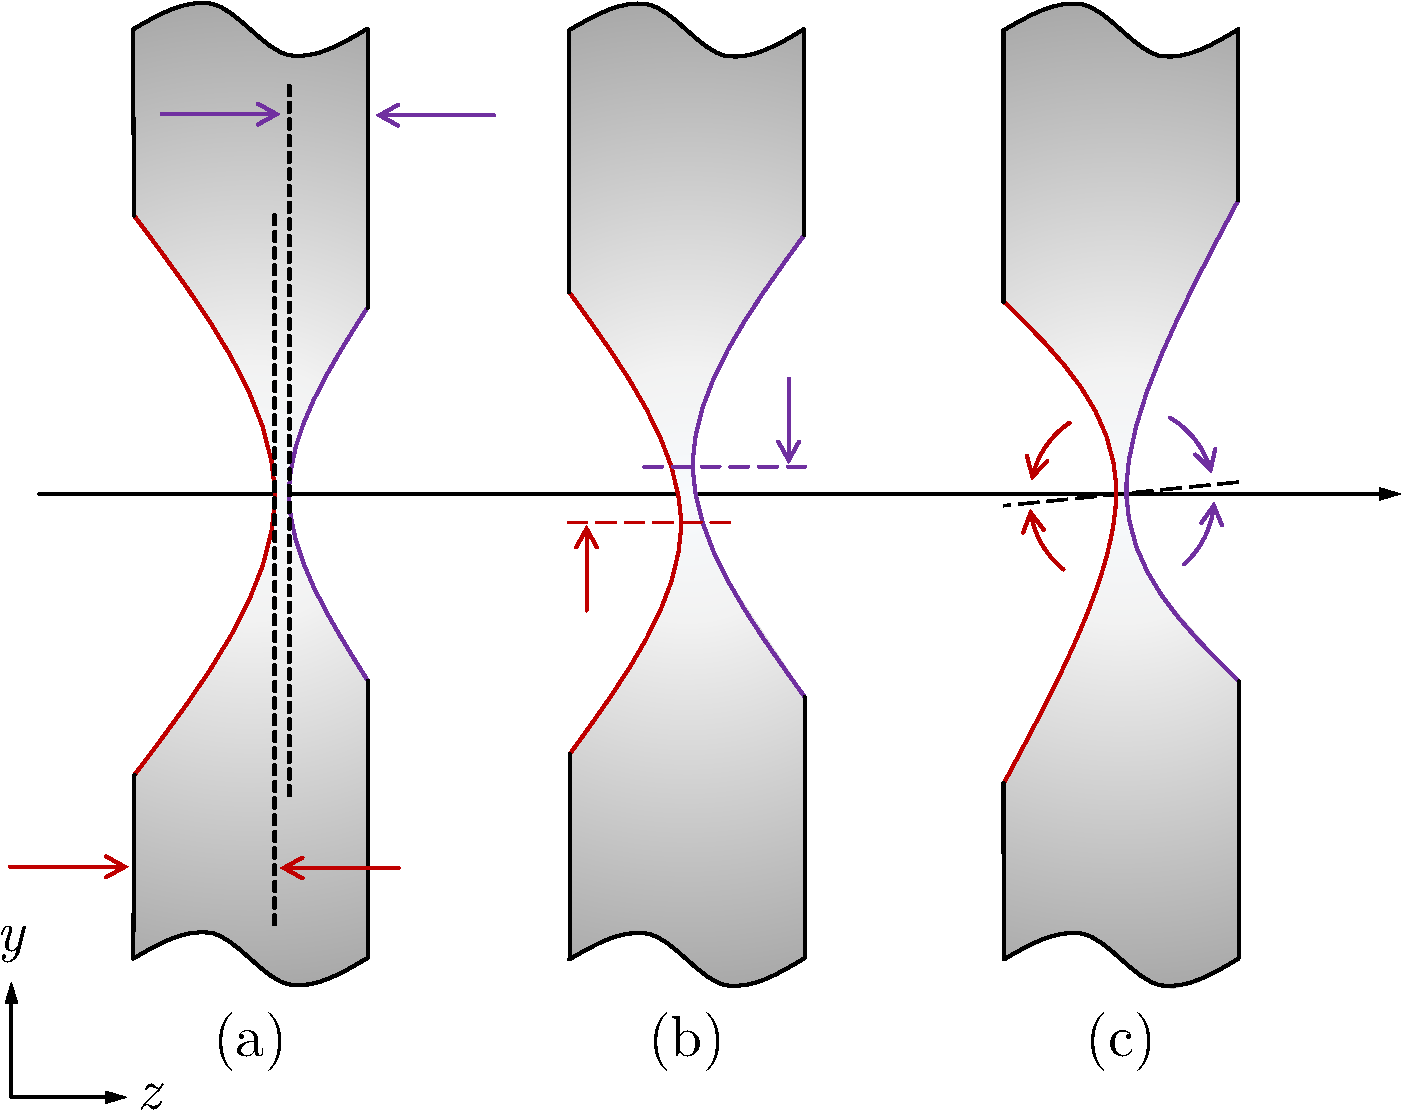
\includegraphics[width=0.4\linewidth]{figures/ch04/manufacturing.pdf}}
    \caption[Typical fabrication errors of bi-concave lenses]{Typical fabrication errors of bi-concave lenses. }
    \label{fig:manufacturing}
\end{figure}

The modelling presented here is general enough to be relevant to most lenses, regardless of fabrication method and, therefore, is not an exhaustive list. 



%-------------------------------------------------------------------------
%-------------------------------------------------------------------------
\subsubsection*{Longitudinal offsets}
%-------------------------------------------------------------------------
%-------------------------------------------------------------------------

Longitudinal offsets of ideal lenses surfaces (shown in Fig.~\ref{fig:manufacturing}(a) do not affect the parabolic accumulated shape a single lens and, consequently, do not impose any optical imperfection to an optical system on based on CRL. However, this lack of symmetry can be often encountered in real lenses\footnote{Specially in embossed lenses, where different penetration depths of the punches often lead to asymmetric lenses.} and due to their 

%-------------------------------------------------------------------------
%-------------------------------------------------------------------------
\subsubsection*{Transverse offsets}
%-------------------------------------------------------------------------
%-------------------------------------------------------------------------

From the point of view of the accumulated thickness in projection approximation, the transverse shift of the two parabolic surfaces behave as the case of two off-set lenses in close contact as described in .

%-------------------------------------------------------------------------
%-------------------------------------------------------------------------
\subsubsection*{Angular offsets}
%-------------------------------------------------------------------------
%-------------------------------------------------------------------------

%-------------------------------------------------------------------------
%-------------------------------------------------------------------------
\subsubsection*{Other sources of deviations from the parabolic shape}
%-------------------------------------------------------------------------
%-------------------------------------------------------------------------

\todo{Discuss half parabolas far and near}

In fact, any (unintentional) deviation of a parabolic shape can be considered as a source of manufacturing error. Each manufacturing process has some type of (signature) error associated to it and with the increasing number of exotic - or non-conventional - designs and tailored manufacturing strategies, it is virtually impossible to create a universal model.

The lack of feasibility in writing a universal model accounting for all possible degrees of freedom errors could have , allied with fabrication errors of a random nature strength the necessity of being able to no only be able to \todo{Link to metrology}

%-------------------------------------------------------------------------
%-------------------------------------------------------------------------
\section{Measuring optical imperfections in refractive lenses}
%-------------------------------------------------------------------------
%-------------------------------------------------------------------------

The metrology data shown in this section was taken on several beamtimes at the BM05 beamline - ESRF [\cite{Ziegler2004}] (from 2017 to 2018 - before the ESRF long shutdown for the EBS upgrade), at the 1-BM beamline - APS [\cite{Macrander2016}] (in 2019 during the ESRF long shutdown) and at the ID06 beamline - ESRF [\cite{Kutsal_2019}] (in 2020 in the commissioning period of the ESRF-EBS upgrade)\footnote{Acknowledgements to Sébastien Bérujon and Ruxandra Cojocaru (BM05-ESRF); Xianbo Shi, Zhi Qiao, Michael Wojcik and Lahsen Assoufid (1-BM-APS-ANL); and to Carsten Detlefs (ID06-ESRF) for the help during the beamtimes.}.%at the ESRF, France, before the ESRF-EBS upgrade shutdown (XX/12/2018)

%-------------------------------------------------------------------------
%-------------------------------------------------------------------------
\subsection{At wavelength-metrology}
%-------------------------------------------------------------------------
%-------------------------------------------------------------------------

%-------------------------------------------------------------------------
%-------------------------------------------------------------------------
\subsubsection*{X-ray speckle tracking}
%-------------------------------------------------------------------------
%-------------------------------------------------------------------------


%-------------------------------------------------------------------------
%-------------------------------------------------------------------------
\subsubsection*{Experimental setup}
%-------------------------------------------------------------------------
%-------------------------------------------------------------------------


[\cite{Berujon2020a, Berujon2020}]


%-------------------------------------------------------------------------
%-------------------------------------------------------------------------
\subsubsection*{Data processing and analysis}
%-------------------------------------------------------------------------
%-------------------------------------------------------------------------

%-------------------------------------------------------------------------
%-------------------------------------------------------------------------
\subsubsection*{Recommended literature}
%-------------------------------------------------------------------------
%-------------------------------------------------------------------------

At-wavelength-metrology, a niche-applicaiton of wavefront sensing, is a vast subject and it is out of scope to discuss in details all the most relevant literature available mainly due to its granularity. Current at-wavelength techniques used for evaluating the phase errors of CRLs (or individual X-ray lenses) are the Ronchigram [\cite{}], a technique based on ...; ptychography [\cite{}] ...; grating interferometry and all its variations [\cite{,,,,}] and speckle-tracking-based methods [\cite{,,,,}].

%-------------------------------------------------------------------------
%-------------------------------------------------------------------------
\subsection{Single lens measurements}
%-------------------------------------------------------------------------
%-------------------------------------------------------------------------

%-------------------------------------------------------------------------
%-------------------------------------------------------------------------
\subsection{Stacked lenses measurements}
%-------------------------------------------------------------------------
%-------------------------------------------------------------------------

%-------------------------------------------------------------------------
%-------------------------------------------------------------------------
\subsection{Corrective optics}
%-------------------------------------------------------------------------
%-------------------------------------------------------------------------

% %-------------------------------------------------------------------------
% %-------------------------------------------------------------------------
% \section{BARC4REFRACTIVE\_OPTICS}
% %-------------------------------------------------------------------------
% %-------------------------------------------------------------------------

$\blacksquare$
\addcontentsline{toc}{section}{References}
\printbibliography[heading=subbibliography]
\end{refsection}

